\section{Introduction}

These notes are personal (subjective) notes about different topics connected to
chromatography modelling. It is like an collage comprised from different
snippets theory snippets.

Some facts may be wrong, therefore please be critical during the usage of the
notes. Any caught mistakes and suggested corrections will be highly appreciated.

\section{Column characterization}
\subsection{Pore size distribution notes}

See Fabi article.

One of the key property of the packed chromatographic columns is its pore size
distribution (PSD). The packed column consists of porous spherical beads (we
assume those are rigid) squeezed together in a cylindrical shaped housing
conventionally called column.

When liquid (usually water solution) travels through such column any
dissolved particles enter and exit pores by means of diffusion, convection or
mass transfer. If we neglect any interaction of particles with the surface of
beads or work in non-binding conditions, particles that enter pores less often
or less deep will travel through the column faster. On the other hand particles
that can reach deep inside many of the pores will travel along the column
slower and thus reach the end of the column at latter time or volume.

Just as a side note, if the conditions are not perfectly non binding, then
exclusion, besides steric basis, may also arise due to: 
\begin{itemize}
    \item if one component is more strongly retained than
    other it will be unable to displace first component and thus won't be able to
        interact with surface.
    \item if component is charged with the same sign as the surface the
        particles will have difficulties entering pores due to Donnan effect.
\end{itemize}

Particle size as well as pore size both play major part in this size exclusion
process. Thus, in order to properly model flow of any particle (even the ones
that have strong interactions with the surface chemistry), having deep
knowledge about PSD is critical.

One way to experimentally determine PSD is to probe the column with
non-interacting particles of different but well known sizes. Very efficient and
well-behaved molecules that are often utilized in such column scrutinization
are Dextrans\footnote{Dextran is a complex branched glucan (polysaccharide
derived from the condensation of glucose), originally derived from wine.} 
of different sizes.

% TODO (ljeromel): Matic add table of dextrans.

For example Dextran-blue (mass of) is regularly utilized to determine
extraparticle volume void (extraparticle porosity).

Let us first define retention (elution) volume. Retention volume of a component 
is the volume after which the component It is measured from the point when
sample with the component is applied to the top of the column and to the point when that
specific component flows out of the bottom of the column. We will denote this
with $V_m$, $m$ as a probing molecule rather than c for component which would collide
with the column :).

Within the chromatographic column there are three characteristic volumes:

\begin{itemize}
    \item Total column volume $V_c$ - volume of the empty "glass" cylinder which is
        used as the column housing and into which we pack the resin beads. 
    \item Extra particle void volume $V_0$ - empty volume between the
        particles. It is the empty volume of the packed colum if particles
        wouldn't be porous (full beads).
    \item Intra particle void volume $V_{p}$ - empty volume within all beads.
\end{itemize}

The intra particle void volume $V_{p}$ is actually sum of all void volumes of
each individual bead, $V_{pi}$:

\[V_p = \sum_{i}^{N}V_{pi},\]

where $N$ is total number of particles within the column (usually this is not
known and almost impossible to determine.


\begin{figure}[h]
	\centering
    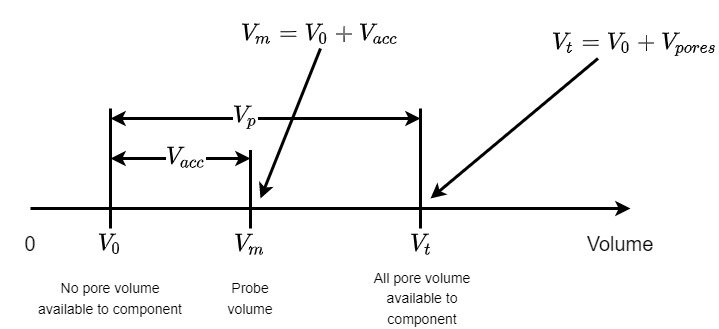
\includegraphics[width=0.7\textwidth]{SEC_volume.jpg}
    \caption{$V_0$ is the column void volume available to all molecules
    (including very large ones). $V_t$ is the total void volume which is $V_0$
    and all void volume in bead's pores. Molecule which can fit into some}
	\label{fig1}
\end{figure}

We assume that due to the size of probe molecule all extra-particle volume is 
available but it can permeate only part of the inter-pore volume,$K$ is a proportional factor which describes how much 

\begin{figure}[h]
	\centering
    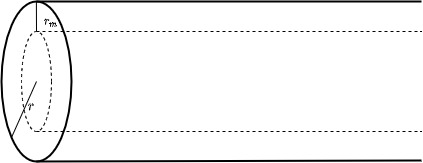
\includegraphics[width=0.4\textwidth]{probe_accessible_vol.jpg}
    \caption{$V_0$ is the column void volume available to all molecules
    (including very large ones). $V_t$ is the total void volume which is $V_0$
    and all void volume in bead's pores. Molecule which can fit into some}
	\label{fig1}
\end{figure}

Accessible volume for spherical probe molecule with radius, $r_m$ and 
infinite cylindrically shaped pore with radius $r$ is:
\begin{equation} \label{eq:acc_vol}
    V_{acc}(r, r_m) = \pi (r - r_m )^2 * L
\end{equation}

\begin{equation}
    V_{pore} = \pi r^2 * L
\end{equation}

Local exclusion factor is thus:
\begin{equation}
    K = \frac{V_{acc}}{V_{pore}} = \frac{\pi (r-r_m)^2 L}{\pi r^2 L} = \left(1 -
    \frac{r_m}{r}\right)^2
\end{equation}

If we are a bit more accurate, and include case when probe molecule radius is
larger than pore we get following
\begin{equation}
	K(r, r_m) = 
	\begin{cases}
        \left(1 - \frac{r_m}{r}\right)^2 & r_m < r,  \\
		0           & r_m \geq r
	\end{cases}
\end{equation}



Main contributions to the dose rate in equation \ref{eq:TG43_basic} are:

\appendix

\section{Glossary}

Here one may find few common but also prone to raise a confusion terms, which
are grouped together in a meaningful way  order to elevate understanding and 
memorization of those.


Some commonly used Latin prefixes:
\begin{itemize}
    \item \textbf{extra-} or \textbf{extro-} - outside (slo. zunaj) - extra-particle volume
    \item \textbf{inter-} - between or among (slo. med) - inter-particle volume,
        inter-molecular bonds.
    \item \textbf{intra-} - within (slo. znotraj) - intra-particle volume,
        intra-molecular bonds.
\end{itemize}


